%!TEX root = ../thesis.tex
%*******************************************************************************
%*********************************** Seventh Chapter *****************************
%*******************************************************************************

\chapter{Correlations of the iPG amplitude wave and Doppler ultrasound, PPG and LDF}  %Title of the First Chapter
\label{chapter correlations}
\ifpdf
    \graphicspath{{Chapter9/Figs/Raster/}{Chapter9/Figs/PDF/}{Chapter9/Figs/}}
\else
    \graphicspath{{Chapter9/Figs/Vector/}{Chapter9/Figs/}}
\fi

Previous chapters provided details about the performance of the designed impedance plethysmography device as well as collected data in resistivity value along with its equivalent in blood flow. The capability of this instrument to detect the changes during the three different kinds of occlusion was also highlighted. Furthermore, the chapters also presented the data collected from other devices such as Doppler ultrasound, LDF, PPG and ECG. 

In this chapter, the correlation between the different measurements will be analysed. The endeavour of this investigation is to understand the contributing factors of the potential impedance plethysmography signal. As explained in previous chapters, the change of volume in the forearm section allowed the estimation of blood flow from the segment. However, both arterial and venous blood contributes to the information of blood flow that was calculated by the iPG device. The extent of blood flow belonging to any blood type remains ambiguous. Besides, it was evident that the main blood vessels contribute to the measurement of blood flow, although microcirculation might also be able to provide additional information under the iPG waveform. 

\section{Analysis of the heartbeat detection in the frequency domain} %Section - 6.1
\label{section correlation 1} 

The signals obtained from each device throughout the experiment are synchronous with the heartbeat. Due to this synchronisation, the systolic peak is also present in the waveform of these instruments in their dynamic component.

Nonetheless, some noises do have a negative impact on the proper detection of systolic peaks carried out during the study. The designed algorithm can detect the shape of the waveform by finding the signal's foot and peaks. Nevertheless, some of its peaks might be missing due to the noise levels.

A Fast Fourier Transform was used to detect the waveforms' main harmonic in a random window data set. The data was selected between \SIrange{580}{780}{\second} for the AC components only, hence the data from $Z_{AC}$ channel. The algorithm was programmed to detect the frequency peak ($f_p$) from \SIrange{0.85}{1.75}{\hertz}. Meanwhile the FFT was limited to detect the frequencies between \SIrange{0}{5}{\hertz} owing to the filters applied to the waveforms, as explained in section \ref{section material envelope}.

From Figure \ref{fig:fft signals} the frequency components from all the participants' measurements can be seen. The ECG plots illustrate the frequency response that is typical of such a signal. Some signals presented a high level of high-frequency components such as the ones witnessed in participants 1 and 8. Participant 3 illustrated a high \SI{2}{\hertz} harmonic peak whose power was greater than the first harmonic. This response seems odd, but by examining the waveform in detail, it showed a lower Q wave which might influence the abnormal frequency component presented in the graph.

\begin{figure}[!htpb]
	\includegraphics[width=1\textwidth,keepaspectratio,trim={0.75cm 0cm 2cm 2cm},clip]{figure1}    
	\caption[Fequency components of the signals acquired]{Fast Fourier transform for all the measurements in the study. Any DC level was removed previous the FFT. The main harmonic represents the heart frequency. The data range corresponds to the time between \SIrange{580}{780}{\second} for the AC components at the measurements.}
	\label{fig:fft signals}
\end{figure}

The iPG device had a mixed frequency response to detect the cardiac heartbeat. As can be seen from the shown plots, some signals exhibit a low-frequency noise which, in some cases, is bigger than the first expected harmonic. For instance, participants 1, 3 4 and 6 found it difficult to detect the frequency peak related to the cardiac cycle for this particular data set. However, the remainder of partakers registered a frequency peak at a similar heartbeat like the ECG. 

PPG frequency components were quite evident in all participants. Some of them showed a high-frequency noise, such as participant 8. However, this signal generally shows low signal to noise ratio in comparison to iPG, which is understandable, as the PPG-AC is significantly bigger than the iPG-AC amplitude.

Lastly, DU exhibited clear FFT components in most participants. Only Participant 1 demonstrated a high noise component in his measurements; the rest showed a response that was similar to the ECG. 

Table \ref{tbl:fft} demonstrates how close the cardiac frequency is to each instrument. However, the iPG mean harmonic and frequency distribution from participant 8 clearly shows that his data was not clean.


\begin{table}[!htbp]
	\caption[Peak frequency obtained from Fast Fourier Transform]{Cardiac frequency obtained from the Fast Fourier Transform for each of the instruments used during the experiment. This peak corresponds to the one with in the hearth cycle in the study (\SI{0.5}{\hertz} < $f_p$ > \SI{1.5}{\hertz})}
	\label{tbl:fft}
	\centering 
	\begin{tabular}{lccccc}
		\toprule
		& \textbf{ECG}
		& \textbf{iPG}
		& \textbf{PPG}
		& \textbf{LDF}
		& \textbf{DU} \\
		& \textbf{$f_p$ [\si{\hertz}]}		
		& \textbf{$f_p$ [\si{\hertz}]}		
		& \textbf{$f_p$ [\si{\hertz}]}
		& \textbf{$f_p$ [\si{\hertz}]}
		& \textbf{$f_p$ [\si{\hertz}]}\\\midrule
		Participant 1    &     0.967    &     0.952    &     0.949    &     0.897    &     0.949    \\  
		Participant 2    &     0.964    &     0.964    &     0.989    &     0.964    &     0.964    \\  
		Participant 3    &     1.041    &     0.916    &     1.041    &     1.038    &     1.019    \\  
		Participant 4    &     1.425    &     1.437    &     1.422    &     1.321    &     1.425    \\  
		Participant 5    &     0.940    &     0.940    &     0.937    &     0.940    &     0.940    \\  
		Participant 6    &     1.239    &     1.242    &     1.242    &     1.233    &     1.239    \\  
		Participant 7    &     1.163    &     1.163    &     1.163    &     1.163    &     1.163    \\  
		Participant 8    &     1.346    &     1.401    &     1.337    &     1.367    &     N/A    \\  
		
		\bottomrule
	\end{tabular}
\end{table}

\section{Correlation between iPG, AC waveform and Doppler ultrasound} %Section - 6.2
\label{section correlation 2} 
The Chapter \ref{chapter apa} showed how the waveforms obtained during the course of this experiment changed in amplitude at each occlusive event. By observing the equation \ref{eq:doppler} from the Doppler ultrasound section, it can be surmised that the velocity ($v$) is directly proportional to the Doppler frequency ($f_D$). The remaining terms can be assumed as constant. Subsequently, the same rule holds true when this velocity is converted into blood flow. Equally, the blood flow calculated from this iPG device with equation \ref{eq:bf} signifies a function of $R_B$ that is directly proportional to the impedance waveform's amplitude at the point $L1$ (see figure \ref{fig:markers iPG}) as illustrated by equation \ref{eq:RB}. In other words, the magnitude of both these measurements alters in accordance to the blood flow.

However, the Doppler ultrasound is solely focused on arterial flow over the blood vessel under observation. Instead, iPG records the changes in flow of both arterial and venous circulation in the volume segment under test. Notably, both devices measure blood flow, albeit in a different manner. The Doppler ultrasound requires precision when placing the instrument's head on the patient's skin. The best signal is obtained when the device is kept exactly over the blood vessel. Hence, the clarity is predicated on the operator's skills to maintain a constant angle and always over the artery. During the course of the experiment, this procedure was replicated using laboratory instruments, keeping angle and skin contact constant. However, using this set-up does not counter rest the participant's arm movement, which causes a misalignment of the sensor. Consequently, the amplitude of this ultrasound signal is not as steady as one might expect. 

As was observed in section \ref{section correlation 1} the AC components of the iPG device are not clean of noise among all partakers. In fact, participant 2, 5, 6 and 7 showed the best signals to work with. For this reason, the waveforms from these partakers were used when performing the correlation between both instruments. 

Figure \ref{fig:corr FWUS} shows the correlation between iPG and DU. The data range corresponds to the entire duration of the experiment and includes the changes of blood flow caused by the occlusions. In the plot, this data was discriminated with a different marker point and colour in accordance to every event during the test. It can be noted that odd regions are baselines, and even regions are blockages.  


The data was normalised and referenced to the highest peak of the total data set.  Each systolic peak detected from the iPG waveform was used to the find the corresponding Doppler ultrasound systolic peak around the same segment of time. Subsequently, the iPG and DU data sets were smoothed by calculating the mean value of every 20 peaks detected within a non-cumulative average.  

The method for analysing the correlation of both measurements was proposed by Bland et al.~\cite{bland1986statistical}. It allows for the comparison of a traditional technique with a new method. Hence, it is ideal to compare the measurements between DU and the designed device. This technique is mostly used to compare similar unit measurements. For this reason, the data were normalised. Therefore, the comparison will be made on the change of magnitude undertaken between both modalities.

On the left side of the plot, the result of the linear regression between both waveforms can be seen. At a certain degree, the data trend is off the line of equity (dotted line), implying that there is no perfect agreement between the two methods concerning their amplitudes. As a matter of fact, this graph shows the linear correlation between both signals with a coefficient correlation of $r^2 = 0.35$ to confirm a link between both signals. However, there is an absence of perfect alignment of the reference signal's (DU) variability alongside the y-axes. 

Analysing region by region illustrates how the data points were distributed along the correlation graph. For instance, there seems to be a good data distribution in both axes throughout regions 1 and 2. It is evident that both waveforms amplitudes spread quite uniformly. Region 1 appears to be closer to the line of equity than region 2 when venous occlusion took place. Apparently, the magnitude of DU signal did not change when compared to the iPG's ones. Undeniably, the impedance plethysmography device detected changes that could not be noticed by DU, which is in agreement as the venous occlusion does not alter the arterial flow. 

\afterpage{
\begin{landscape}
	\centering
	\vspace*{\fill}
	\begin{figure}[!h]
		\includegraphics[width=1.33\textwidth,keepaspectratio]{figure2}    
		\caption[Bland and Altman plot of the relation between Doppler ultrasound and iPG]{Bland and Altman~\cite{bland1986statistical} plot of the relation between Doppler ultrasound and iPG. Data set corresponds to participants 2, 5, 6 and 7. The data has been normalised comparing the amplitude of both measurements. The different regions have been plotted with various colours and symbols to differentiate every event. The dotted line represents the perfect agreement; the dark line is the linear regression.}
		\label{fig:corr FWUS}
	\end{figure}
	\vspace*{\fill}
\end{landscape}}

However, region 3 shows a bigger distribution of data points (than iPG) adjacent to y-axes. It is possible that the participants' movements caused this significant variation of the DU amplitude. By reviewing the envelope of signal illustrated in figure \ref{fig:DU flow} it can be seen that Participant 7 showed the largest waveform amplitudes; this can also be confirmed in the mean blood flow computed on the same region. In fact, the linear regression improves to $r^2 = 0.45$ when the data was run without this participant. 

Region 4 demonstrates a similar behaviour as region 2; there is a good amount of data distribution, but the iPG amplitude changes more than the DU. Notably, there is a greater concentration of data points in the lower region of both axes. However, this is expected as there is a reduction of arterial blood during this event. The higher data points towards the iPG axes pertain to the blood flow rush towards the beginning of the occlusion on participant 7, which is illustrated in \ref{fig:blood_flow_plethysmography}.

Region 5 shows a higher distribution of the data adjacent to the iPG axes. On the other hand, some data points on the lower part of the DU axes impact the linear regression in this region. During total occlusion occurring in region 6, the DU device witnesses a better response. Here, a significant number of the Doppler's ultrasound data points are set to zero, whereas the data from iPG is mostly distributed among 0 and 0.2. Finally, region 7 exhibits a good distribution that is adjacent to the line of equity, which is in congruity with some of the other baseline behaviours.

The plot on the right side of figure \ref{fig:corr FWUS} shows the precision between the estimated limits of agreement of the experiment.  On the y-axes, the mean difference between the two measurements and the points of its standard deviation is plotted. The differences have normally been distributed in a Gaussian space. Hence, \SI{95}{\percent} confidence interval of the difference should be located between $\pm 1.96$SD. This graph shows a high number of points out of $+ 1.96$SD. However, it can be seen that values from regions 2 and 4 are outside of the agreement region. This confirms that when an occlusion occurs, there is a different response between iPG and DU.


\section{Correlation between iPG and PPG}  %Section - 6.3 
\label{section correlation 3}
The correlation between iPG and PPG was also investigated when looking for amplitude similarities between both signals during the occlusive events. In a similar manner, the method used in the previous chapter was used here as well in order to analyse the change of magnitude between both AC waveforms. The two signals represent the changes of volume within a part of the body, PPG in the finger and iPG in the forearm. Although the PPG reflects blood movement within the blood vessels beneath the skin in a not so well-defined volume \cite{elgendi2012analysis}, iPG provides crucial information about the change of volume by the blood vessels being filled with blood but limited by the sensing electrodes.

However, the PPG method used in this study was very simplistic when compared to more sophisticated methods that may be able to detect the changes in venous and arterial flow using other wavelengths, sensor placement, or data interpretations. The correlational study of this section looks to decipher the changes in amplitude among AC components of both signals. As detailed in previous chapters, both signals illustrated changes within their DC components for the time that they were occluded. However, the AC component of both signals changed oppositely. While there was a magnitude increment in the iPG waveform all along the occlusions (see figure \ref{fig:blood_flow_plethysmography}), the PPG waveform (see figure \ref{fig:RED PPG}) witnessed a decline in amplitude during these events.

As shown in figure \ref{fig:blood_flow_plethysmography} participant 2 displayed abnormal AC amplitudes during the time of this experiment. Also, detailed in the previous section, participants 2, 5, 6 and 7 showed a better AC response. It is for this reason that the data of participant 2 was excluded from the correlation between these two waveforms. The data sets were smoothed by calculating the mean value of every 20 peaks in a non-moving average.

\afterpage{
\begin{landscape}
	\centering
	\vspace*{\fill}
	\begin{figure}[!h]
		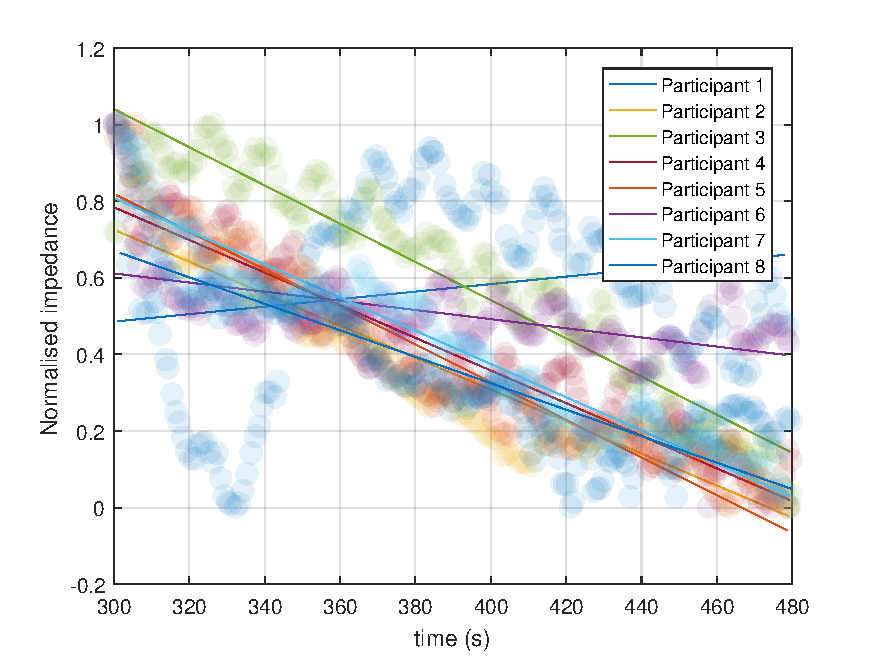
\includegraphics[width=1.33\textwidth,keepaspectratio]{figure3}    
		\caption[Bland and Altman plot of the relation between PPG and iPG]{Bland and Altman~\cite{bland1986statistical} plot of the relation between PPG and iPG. Data set corresponds to participants 5, 6 and 7. The data was normalised comparing the amplitude of both measurements. The different regions have been plotted with various colours and symbols to differentiate every event. The dotted line represents the perfect agreement, and the dark line is the linear regression.}
		\label{fig:corr RED}
	\end{figure}
	\vspace*{\fill}
\end{landscape}}

The Bland et al.~\cite{bland1986statistical} statistical analysis was also implemented in this study. Figure \ref{fig:corr RED} shows the correlation between iPG and PPG magnitudes. The chart on the left shows the absence of a perfect correlation during the study, which was expected because the signal's amplitude goes in opposite directions all along the venous and arterial occlusions. Notably, the graph shows a poor linear correlation between both signals with an $r^2 = 0.07$.

Most of the baseline data points (regions 1,3,5 and 7) are closer to the line of equity. In fact, if the venous and arterial occlusive events were removed, there would be a significant improvement in the correlation between both measurements ($r^2 = 0.40$). By analysing the results of this graph, it can be confirmed that the iPG magnitude changed significantly while PPG's amplitude reduced during the course of venous and arterial occlusions. It is also verified that the PPG amplitude all along the arterial blockage is lower than venous occlusion, as illustrated by the data points in the figure. On the other hand, there was a similar response to both signals at the time of total occlusion, and the absence of blood flow translated into small amplitude values. The PPG data points were closer to zero in comparison to the iPG magnitudes that were closer to \num{0.1}.

The BA (Bland and Altman) plot on the left side of figure \ref{fig:corr RED} illustrates greater precision at the time of these baseline readings. Most of the data points are within the \SI{95}{\percent} confidence interval ($\pm 1.96$SD), while the measurements taken during occlusion were mostly outliers.

\section{Correlation between iPG and LDF}  %Section - 6.4 
\label{section correlation 4}
The signal from the LDF device provides information about the flow movement of red blood cells within the microvascular network under the skin. However, a weak correlation between measurements is not surprising because data errors in this instrument have been widely documented, especially at low blood flow~\cite{perkash1988difficulties}. Another shortcoming of this technique is that it is unclear whether the measurements belong to a venous or arterial flow. 

The position of this LDF sensor head helps understand the blood flow under microvascular bed beneath the forearm. As described in section\ref{section procedure 1.1}, the sensor was placed on the forearm midpoint between the iPG's sensing electrodes. 

The signal coming from the LDF device is similar to a plethysmography wave, which is formed by the AC component on a DC signal. For the purpose of a correlation analysis of this study, the DC component of this signal had to be removed, which only left the comparison between of normalised AC magnitudes of the LDF and iPG signals. Similarly, as evidenced in the previous analysis, the data was smoothed by taking the average value of 20 data points. Finally, the data depicted belongs to participants 2, 5, 6 and 7.

Figure \ref{fig:corr LDF} illustrates the linear regression and BA analysis between both signals. Notably, the data points show a poor correlation among both signals ($r^2 = 0.08$). Most data points are far from the line of equity and mostly spread across the plot x-axis. The data points from this LDF signal are not well scattered around the figure. This imbalance can mostly be noticed in the region 7.  One plausible explanation of this effect is that the LDF peak extension is impacted by the hyperaemic effect upon the release of total occlusion, as can be seen in figure \ref{fig:LDF flow}. Nonetheless, if this data were removed from the plot, there would still be a weak agreement between both signals ($r^2 = 0.08$).

Based on the BA chart on the right side of the figure, poor accuracy is observed when comparing the amplitude of both measurements. Therefore, it is not possible to establish any relation within the magnitude waveform of these two instruments.


\afterpage{
\begin{landscape}
	\centering
	\vspace*{\fill}
	\begin{figure}[!h]
		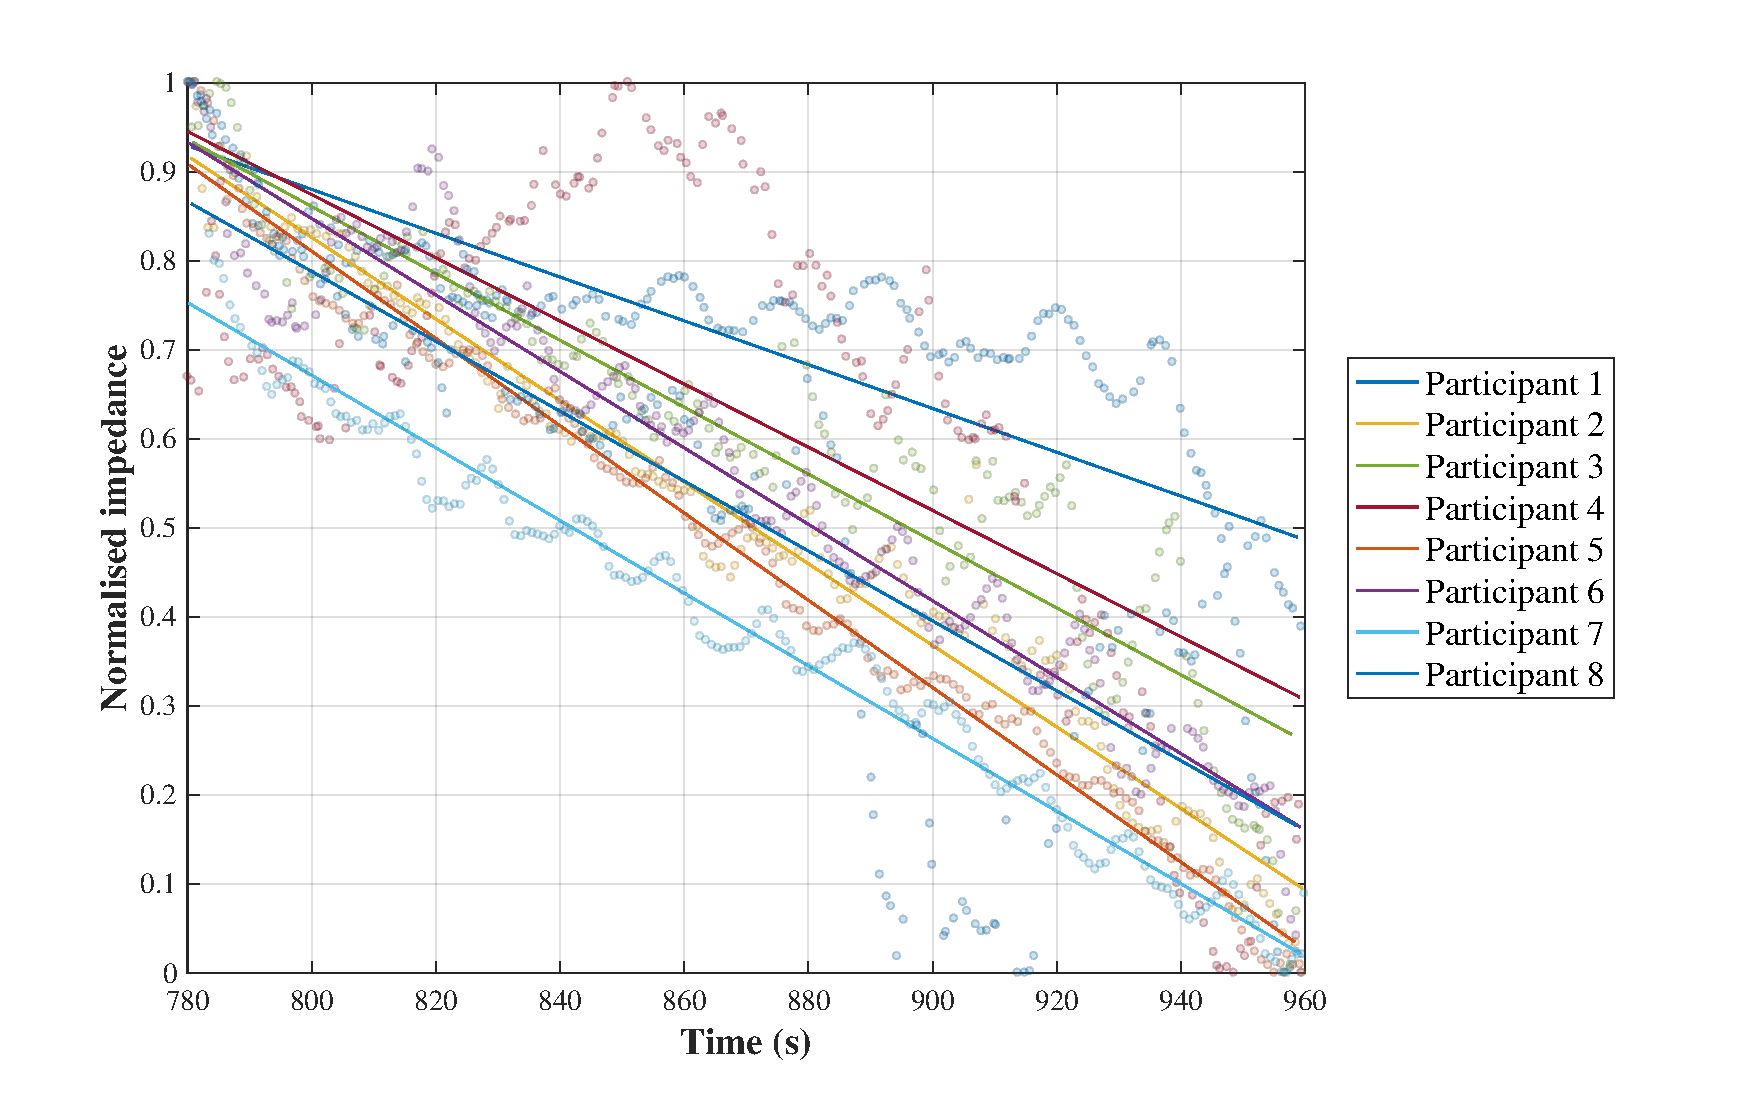
\includegraphics[width=1.33\textwidth,keepaspectratio]{figure4}    
		\caption[Bland and Altman plot of the relation between LDF and iPG]{Bland and Altman~\cite{bland1986statistical} plot of the relation between LDF and iPG. Data set corresponds to participants 2, 5, 6 and 7. The data was normalised when comparing the amplitude of both measurements. The different regions have been plotted with various colours and symbols to differentiate every single event. The dotted line represents the perfect agreement, and the dark line signifies the linear regression.}
		\label{fig:corr LDF}
	\end{figure}
	\vspace*{\fill}
\end{landscape}}

\section{Conclusion}  %Section - 6.5
\label{section correlation 5}
The iPG device provides an AC signal which is synchronous with the heart cycle. In general, the FFT analysis of all participants showed similar harmonics as the ones that were noted by the ECG signal. This effectively means that the iPG changes in accordance to the heart cycles. Nonetheless, only 4 people demonstrated clear signal-to-noise ratio waveform; the remaining ones presented low-frequency noises which decreased their data quality. The nature of these low frequency components remains unknown since the signal was filtered.

A statistical analysis comparing the amplitude of the iPG device with other instruments was performed.  A good correlation between the iPG device and the Doppler ultrasound ($r^2 = 035$) was found. The latter showed better zero sensitivity than the iPG, but when there was a change in the blood flow, the impedance plethysmography device could detect variations in the three kinds of occlusion performed. However, the analysis highlighted a low precision during these occlusive events. 

Meanwhile there was a low correlation with the other two devices - PPG and LDF. In the case of PPG, there was a poor correlation ($r^2 = 0.08$) since its amplitude waveform decreases, while the iPG increased all along the venous and arterial occlusions.  By removing this component, the correlation improved to ($r^2 = 0.40$), but both responded differently when occlusion occurred.

The worst correlation was seen between the iPG and the LDF ($r^2 = 0.07$). Including or excluding the data from the blockage events does not impact this relation. In fact, the movement of RBCs detected by the LDF can hardly be related to the iPG waveforms. This lack of correlation could be attributed to the bigger noise peaks detected on the LDF signal. This can be confirmed when comparing both FFT signals. In most participants, the amount of noise collected by this method diminished the frequency of interest. 

The data correlation between the iPG arterial pulses and other instruments helps us understand the kinds of blood that significantly contribute to the iPG signal. The data from blood flow (per volume of tissue) quantified from the iPG data shown in chapter \ref{section apa flow arterial pulses} highlighted increments in their respective systolic peaks all along venous or partial arterial. Indeed, the systolic pulses during partial arterial occlusion were slightly higher than the ones that occurred during venous occlusion. This information contrasted with the data observed in Doppler Ultrasound measurements. As described in chapter \ref{section comparison 2} the arterial flow was mostly affected when the blockage occurred at a point that was above diastolic pressure. The amplitude of the iPG's systolic pulses was also expected to decrease during disturbances of the arterial flow due to restricted blood flow into the limb, but it actually increased. One explanation could be that the body triggered a vasodilatory response when an occlusion occurred where the veins' cross-section area veins increments to accommodate more blood into the tissue. 

The response seen from the iPG signal is unique since other instruments exhibited a reduction in their systolic peaks in a similar proportion. For instance, as shown in \ref{section comparison LDF} and \ref{section comparison PPG} both signals witnessed a reduction in their amplitudes during venous and partial arterial occlusion. This same response can be attributed to the measurement of changes in the venous blood, but not in the arterial. In fact, the decline in LDF amplitude suggests a reduction in the velocity of RBC coming into the microcirculation. Additionally, this decline of the PPG amplitude is indicative of a shift in blood volume activated by the venous occlusion. During this experiment, the magnitude of PPG reduces significantly during partial arterial occlusion.

In general, it appears as though the arterial blood is a significant contributor of the iPG's APA signal by not merely detecting the arterial blood coming into the limb, but by also giving an insight into how the tissue responded to a blood occlusion. The good correlation with the Doppler Ultrasound  ($r^2 = 0.35$) as shown in chapter \ref{section correlation 2}, illustrated that the iPG waveform amplitude did change with the arterial blood. Nevertheless, while reducing the arterial blood, the forearm's iPG waveform reacted differently, causing a spike in the systolic magnitude possibly because of a venous response.  When correlating the iPG data with PPG (see chapter \ref{section correlation 4}) and LDF (see chapter \ref{section correlation 3}) methods a low correlation was found ($r^2 < 0.08$); this was apparently caused by the different direction that the amplitudes went towards. While the iPG increased, the optical methods decreased. This reaction seems to indicate that the changes occurring in venous blood presented an increase in the iPG amplitude pulses, probably due to an increase in the vessels' diameter during an occlusion.


%********************************** %Nomenclature found  *************************************
\nomenclature[z-ecg]{FFT}{Fast Fourier Transform}
\nomenclature[z-baa]{BA}{Bland and Altman analysis}